\section{Distinguish Devices}
IoT applications utilise a great variation of devices, with each having different processing power. Thus the same operation, e.g. processing a PING packet, takes different time on different devices. This opens the potential of leaking hardware information through observing packet timings.

Although not uniquely, PING is specifically an ideal feature supported in 6LoWPAN that can be exploited to perform such attack due to:
\begin{enumerate}
	\item PING is processed in a highly predictable routine where nearly no computation is required, minimising the noise induced by different data.
	\item The support of PING is required by the IPv6\cite{rfc4443}, making the attack universally applicable.
\end{enumerate}

When using the ping command in Linux distributions, it is recommend to add the ``-s 0'' option to remove the user defined data and thus avoid exceeding 6LoWPAN MTU (127 bytes). The interval option  ``-i'' must also be used with care as excessing frequency may flood the devices and cause inaccurate measurements.

\subsection{Computing PING Response Time}\label{TimingWithContikiMAC}
Contiki adopts a Radio Duty Cycle (RDC) protocol called Contiki MAC\cite{ContikiMAC} to preserve energy. On ther receiver's side, Contiki MAC switching off the radio for most of the times and periodically wakes it up for a short period for signal detection. If a signal is detected during that period, the radio is kept on until the packet is received. On the other hand, the sender repeatedly sends a packet, until one of them is detected by the receiver and the next one being received and acknowledged.

As a result, duplicated packets may be observed in the captured traffic. To best approximate the processing time for a specific PING request, the PING Response Interval (PRI) is defined as the time elapsed between the last PING request being sent and the first PING response being replied. 

\paragraph{Example}

\AddFigure{fig/PRI.png}{PRI Example}{PRIExample}

\Cref{PRIExample} shows an example of packets captured by Wireshark\cite{Wireshark}. Duplicated PING requests, \#$198$ to \#$203$, are replied by a single response, \#$205$, matched by their \textit{seq} field ($=16$). The PRI is therefore computed as the time between \#$203$ and \#$205$ which is:
\begin{equation*}
PRI = 4.701468 - 4.684369 = 0.017099(s) = 17.099(ms)
\end{equation*}

\subsection{PRIs on TelosB and CC2538}

\Cref{PRIs} shows PRIs collected on two devices, TelosB and CC2538, running the same Contiki broadcast example. The graph demonstrates that they can be easily distinguished, as PRIs of TelosB are clustered around $17(ms)$ whilst CC2538 around $10(ms)$.

\begin{figure}
	\begin{subfigure}{0.45\linewidth}
		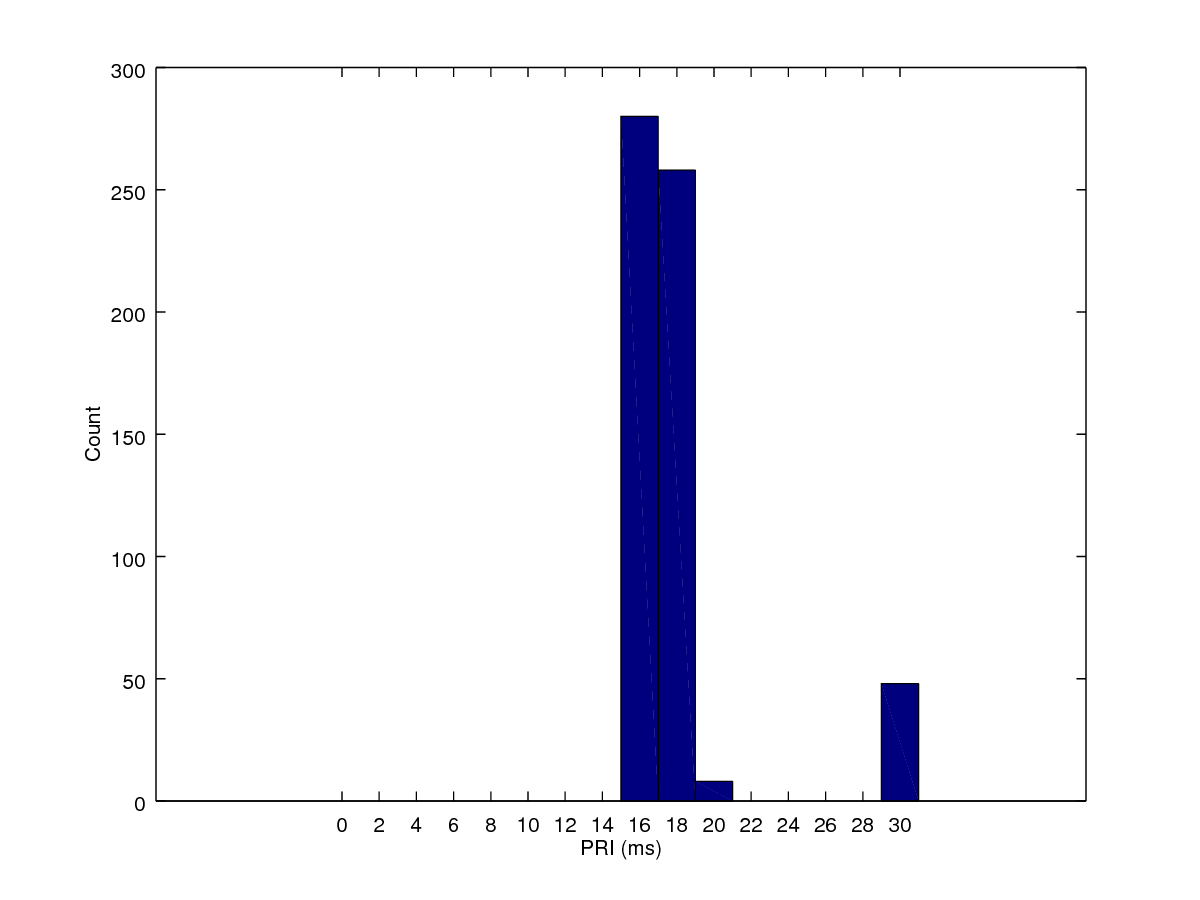
\includegraphics[width=\linewidth]{fig/helloworld_sky.png}
		\subcaption{TelosB PRIs}
	\end{subfigure}
	\begin{subfigure}{0.45\linewidth}
		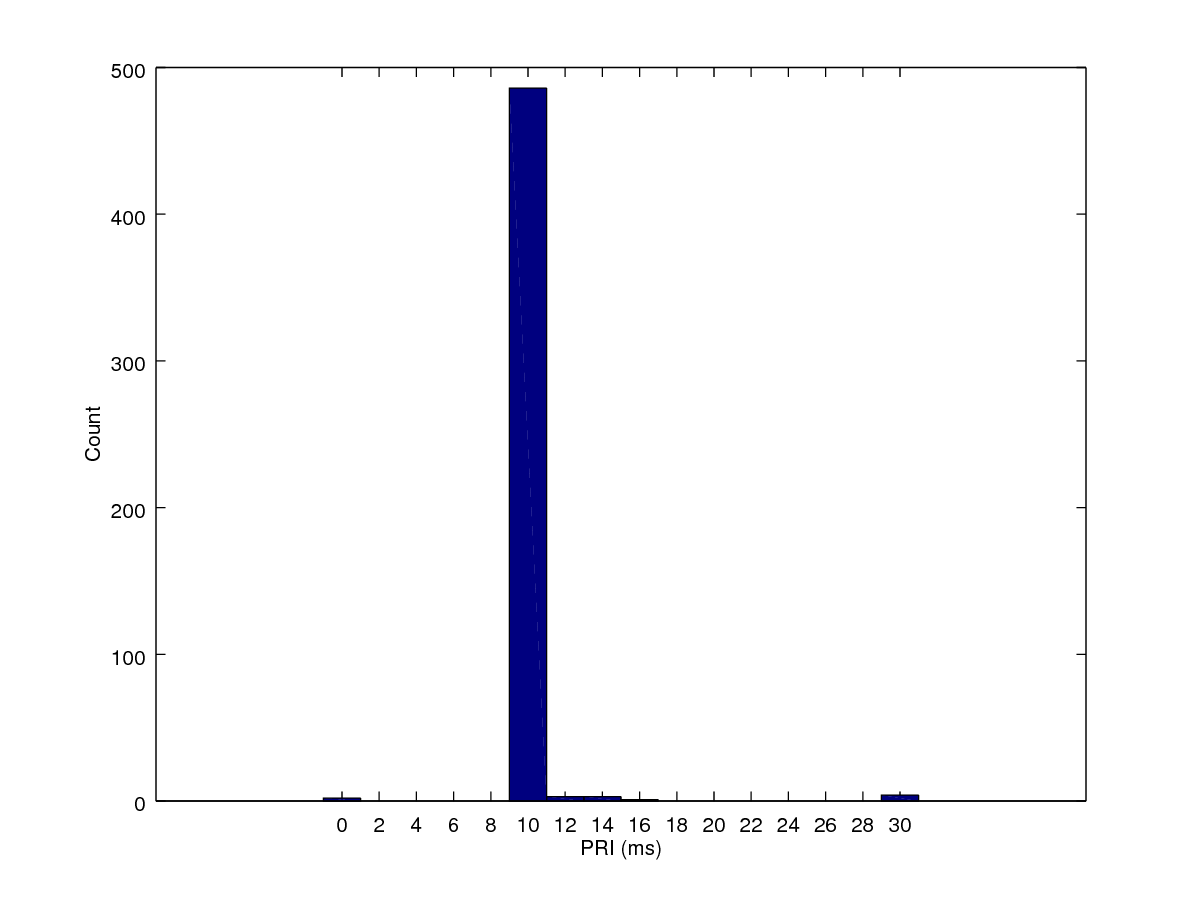
\includegraphics[width=\linewidth]{fig/helloworld_CC2538.png}
		\subcaption{CC2538 PRIs}
	\end{subfigure}
	\caption{PRIs for different devices. \label{PRIs}}
\end{figure}

We also realised that certain outliers exist in the data. A common cause of outliers could be that the CPU was occupied by other tasks when the PING request is received and thus delaying the response. To mitigate the affect of outliers, we propose the use of median to characterise the devices, as summarised in \Cref{PRI_SkyCC2538}.

\begin{table}[ht!]
	\centering
	\adjustbox{max width = \textwidth}
	{
		\begin{tabular}{|c|c|c|}
			\hline
			              & Mean (ms)     & Median (ms)   \\ \hline
			TelosB & 33.818 & 17.033 \\ \hline
			CC2538 & 11.205  & 9.551 \\ \hline
		\end{tabular}
	}
	\caption{PRIs of TelosB and CC2538}
	\label{PRI_SkyCC2538}
\end{table}


\subsection{Factors Affecting PRI} \label{PingDevice}

Many IoT devices provide a sleep mode for energy preserving which usually comes with downgraded performance. As a result, devices tend to have a longer PRI when they are under sleep mode. 

\#SKY broadcast\_example VS powertrace\#

Since nodes tend to remain in sleep mode for most of the time in typical WSN applications, we measured the PRIs under sleep mode to characterise two devices, namely TelosB\cite{TelosB} and CC2538\cite{CC2538}. Optionally for TelosB, the default software AES implementation can be replaced a hardware coprocessor. We demonstrate our result of PRIs on the above platforms in \Cref{PINGTiming}.

\begin{figure}[ht!]
	\centering
	\begin{subfigure}{0.4\textwidth}
	{
		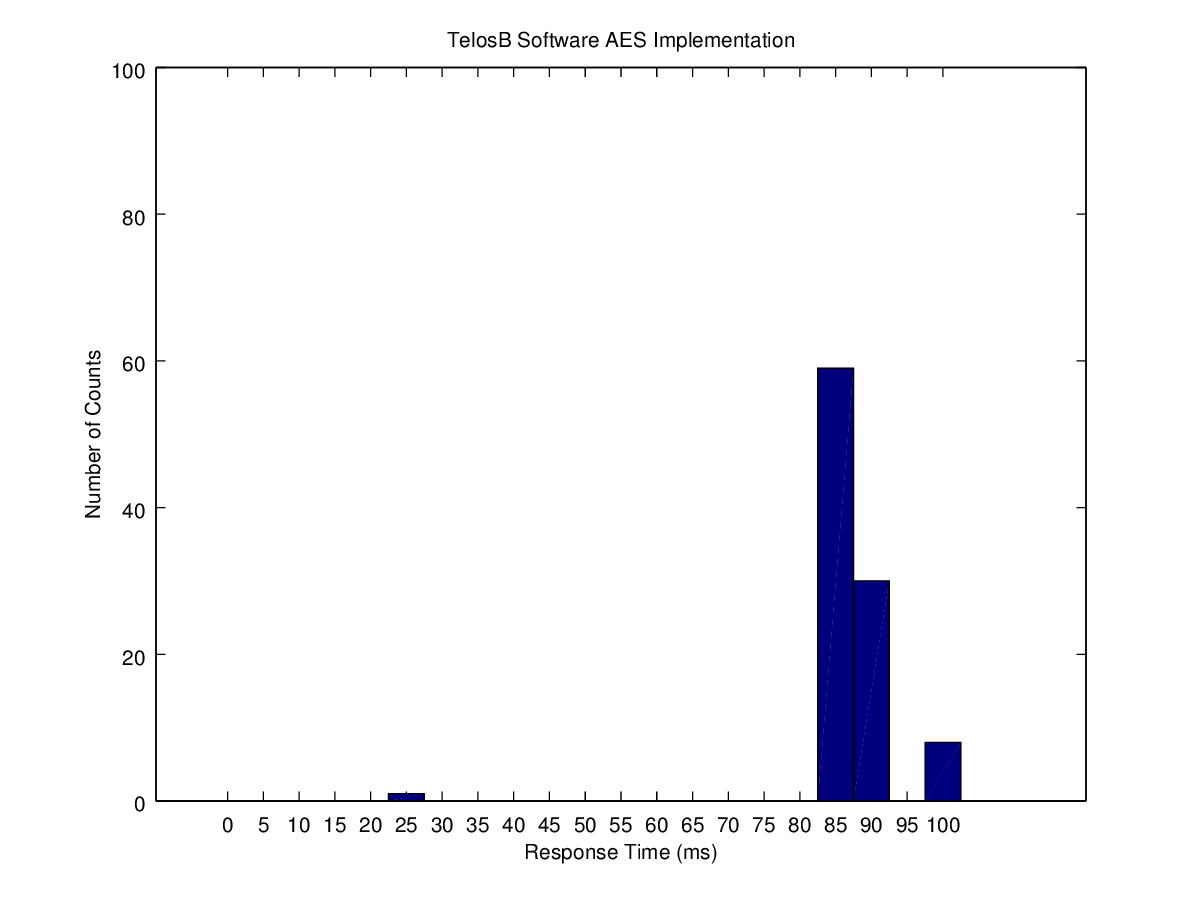
\includegraphics[width=\textwidth]{fig/noncoresec_ping_telosb_sw.png}
	}
	\end{subfigure}
	\begin{subfigure}{0.4\textwidth}
	{
		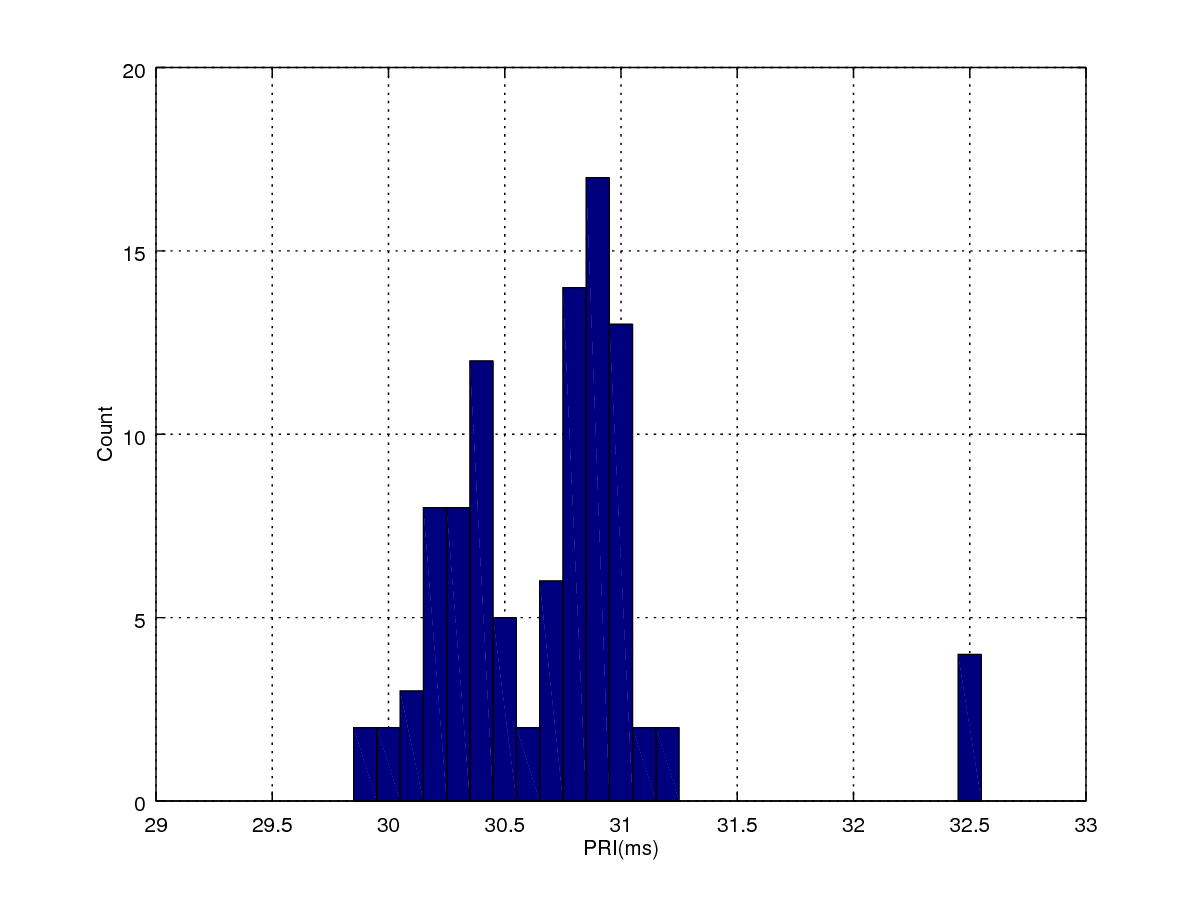
\includegraphics[width=\textwidth]{fig/noncoresec_ping_telosb_hw.png}
	}
	\end{subfigure}
	\begin{subfigure}{0.4\textwidth}
	{
		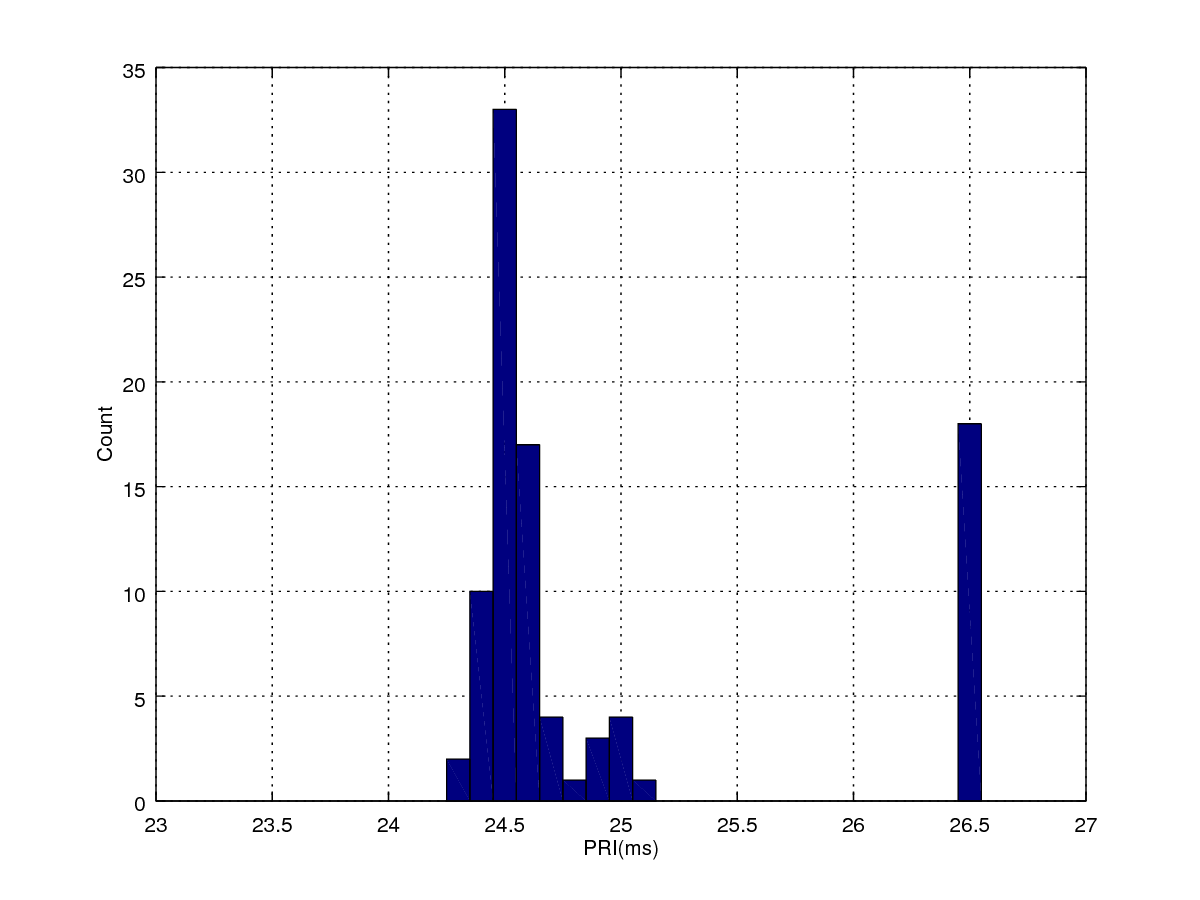
\includegraphics[width=\textwidth]{fig/noncoresec_ping_cc2538_sw.png}
	}
	\end{subfigure}
	\caption{PING Reponse Time for TelosB and CC2538\label{PINGTiming}}
\end{figure}

%Data Analysis
Observing \Cref{PINGTiming}, it is intuitively clear that different devices (and setups) result into different PRIs. 

Not to our surprise, the means and medians are significantly different to each others, as we summarised in \Cref{PINGResponseTimeTbl}. We consider the median as a statistically more effective indicator as it is less affected by the outliers. 

\begin{table}[ht!]
	\centering
	\adjustbox{max width = \textwidth}
	{
		\begin{tabular}{|c|c|c|}
			\hline
			              & Mean (ms)     & Median (ms)   \\ \hline
			TelosB HW AES & 37.20 & 30.77 \\ \hline
			TelosB SW AES & 105.19        & 87.40          \\ \hline
			CC2538 SW AES & 48.83         & 24.55          \\ \hline
		\end{tabular}
	}
	\caption{PING Response Time}
	\label{PINGResponseTimeTbl}
\end{table}

The result indicates that it would be possible to reveal device models (and setups) from the encrypted traffic by simply compare PRIs to profiled data, assuming they are selected from a known set. Combined with the attack in \Cref{ICMPAttack}, one could further apply the similar timing attack on any extractable ICMP messages in the encrypted traffic.